\chapter{Inerciální senzory}
Ke sběru dat pro účely inerciální navigace se jako první začaly používat a stále používají např. v letectví složité, velké a drahé mechanické přístroje se setrvačníky poháněnými motory využívající gyroskopický efekt. Jejich natočení os vůči referenčnímu rámu je poté možné měřit například laserem, či jiným způsobem. Tyto senzory jsou díky jejich přesnosti stále využívány v aplikacích, kde je kladen důraz na opravdu velkou spolehlivost a přesnost. Ovšem díky zlepšujícím se technologiím se začínají hojně využívat i \ac{MEMS} \ac{IMU} v oblastech inerciální navigace, zejména tam, kde nejsou kladeny velmi přísné požadavky na přesnost a spolehlivost, jako je například navigace uvnitř budov. Díky \ac{MEMS} technologiím je možné sestrojit celou inerciální jednotku bez jakýchkoliv pohyblivých částí, velmi malou a poměrně levnou. \cite{Tittertonc2004} \cite{Grewal2013}

\section{MEMS akcelerometry} \label{MEMSaccel}
Akcelerometr měří lineární zrychlení nepřímo díky druhému Newtonovu zákonu (rovnice \ref{eq:2NZ}). Přímo na struktuře křemíku je těleso známé hmotnosti, kterému je umožněn pružný pohyb v nějaké z os. Pokud na akcelerometr působí zrychlení, je těleso vychylováno silou, která je následně měřena. Tato síla je často měřena jako změna kapacity mechanické struktury znázorněné na obrázku \ref{fig:MEMSaccelerometer} a \ref{fig:MEMSaccelerometerPhoto}, převedena na napětí, zesílena, vyfiltrována a následně převedena analogově-digitálním převodníkem (\emph{Analog to Digital Converter}, \acsu{ADC}).
Tyto struktury jsou následně uspořádány ortogonálně, aby vytvořily tříosý akcelerometr. \cite{Dadafshar2014}

\begin{figure}[h]
    \centering
    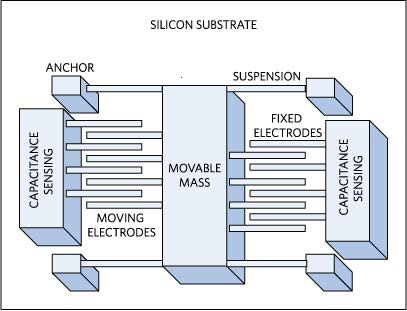
\includegraphics[width=0.5\textwidth]{obrazky/MEMSaccelerometer}
    \caption{Struktura MEMS akcelerometru. \cite{Dadafshar2014}}
    \label{fig:MEMSaccelerometer}
\end{figure}

Za povšimnutí stojí rozdílné parametry např. biasu pro různé osy \ac{IMU} v tabulce \ref{table:fyzikalniPorovnaniIMU}, to může být způsobené vrstvením struktury během výroby čipu, kdy dvě z os akcelerometru mají osy vychýlení hmoty rovnoběžnou se směry vrstev, zatímco třetí osa je na tyto vrstvy kolmá.

\begin{figure}[h]
    \centering
    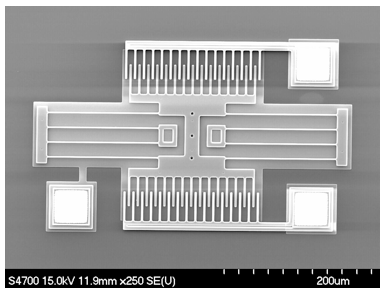
\includegraphics[width=0.5\textwidth]{obrazky/MEMSaccelerometerPhoto}
    \caption{Mikroskopický snímek MEMS akcelerometru. \cite{cCumN04KaPNjERaF}}
    \label{fig:MEMSaccelerometerPhoto}
\end{figure}

\section{MEMS gyroskopy}
Gyroskopy jsou senzory, které měří úhlovou rychlost. Uspořádání mechanické struktury (na obrázku \ref{fig:MEMSgyroscope}) je rozdílné v porovnání s akcelerometry. Zde je tělesu definované hmotnosti umožněno kmitat v jedné z os. Při působení úhlové rychlosti na gyroskop je vnitřní struktura díky Coriolisově síle vychýlena, což způsobí změnu kapacity. Ta je dále zpracována obdobně jako v akcelerometru (kapitola \ref{MEMSaccel}). \cite{Tittertonc2004} \cite{Dadafshar2014}
\begin{figure}[h]
    \centering
    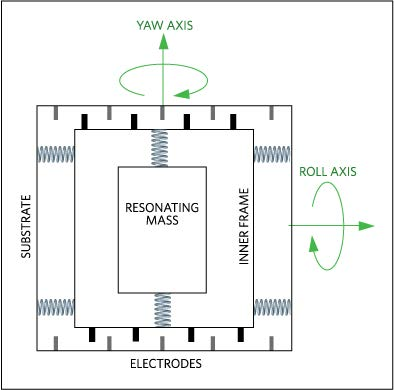
\includegraphics[width=0.5\textwidth]{obrazky/MEMSgyroscope}
    \caption{Struktura MEMS gyroskopu. \cite{Dadafshar2014}}
    \label{fig:MEMSgyroscope}
\end{figure}
